\begin{figure}[htp]
	\centering
	\subfloat[\(\mesh{W^{\Phi}}\)]
	{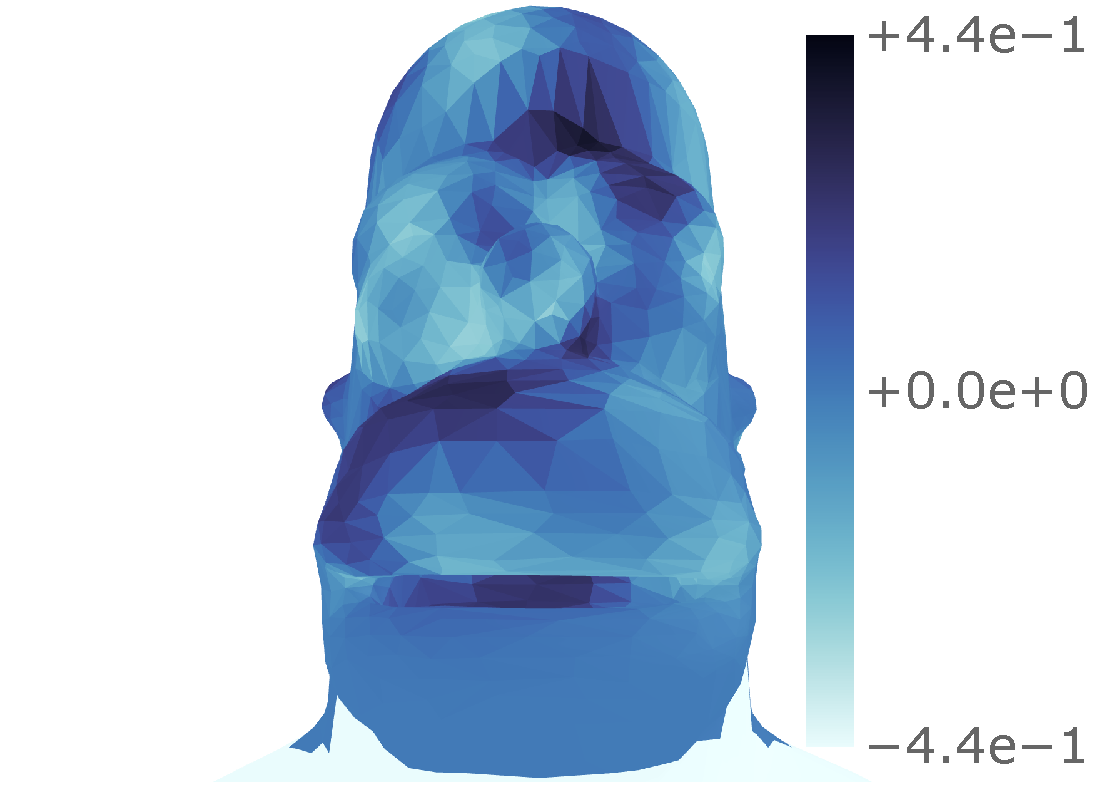
\includegraphics[trim={101 0 3 3},clip,width=.33\textwidth]{slepian_wavelet_coefficients_homer_3B_2jmin_scaling_zoom.pdf}}
	\hfill
	\subfloat[\(\mesh{W^{\Psi^{2j}}}\)]
	{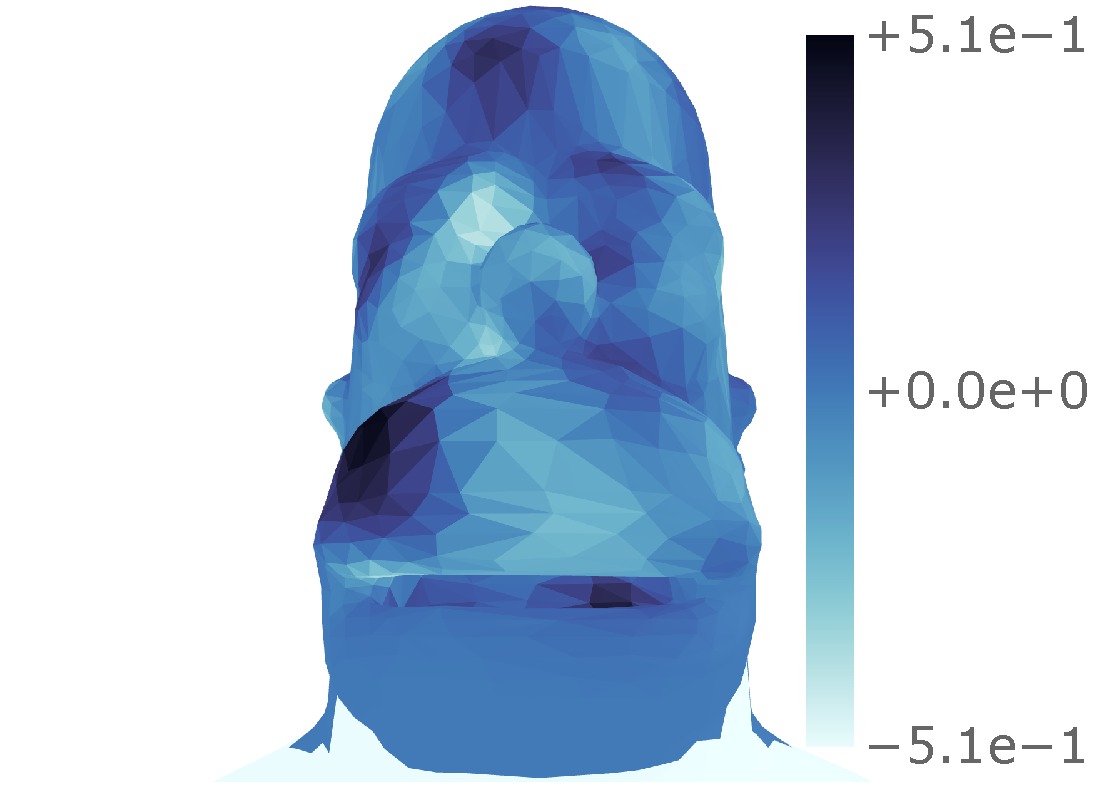
\includegraphics[trim={101 0 3 3},clip,width=.33\textwidth]{slepian_wavelet_coefficients_homer_3B_2jmin_2j_zoom.pdf}}
	\hfill
	\subfloat[\(\mesh{W^{\Psi^{3j}}}\)]
	{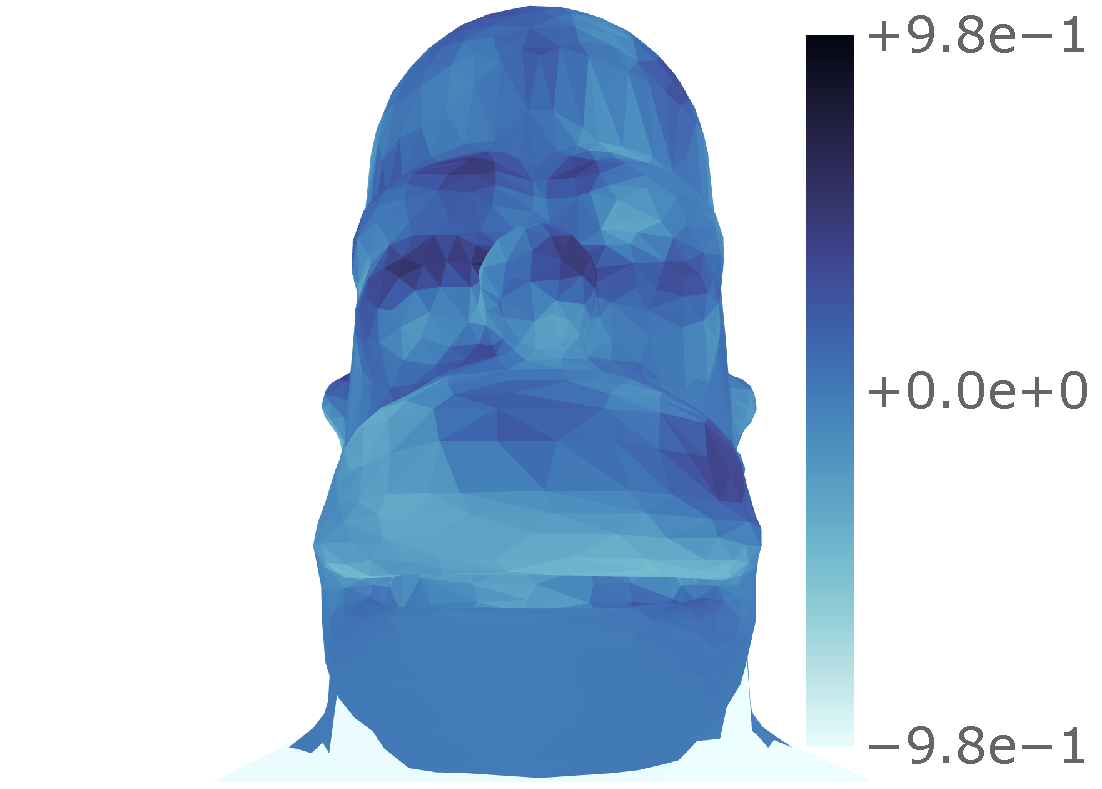
\includegraphics[trim={101 0 3 3},clip,width=.33\textwidth]{slepian_wavelet_coefficients_homer_3B_2jmin_3j_zoom.pdf}}
	\newline
	\subfloat[\(\mesh{W^{\Psi^{4j}}}\)]
	{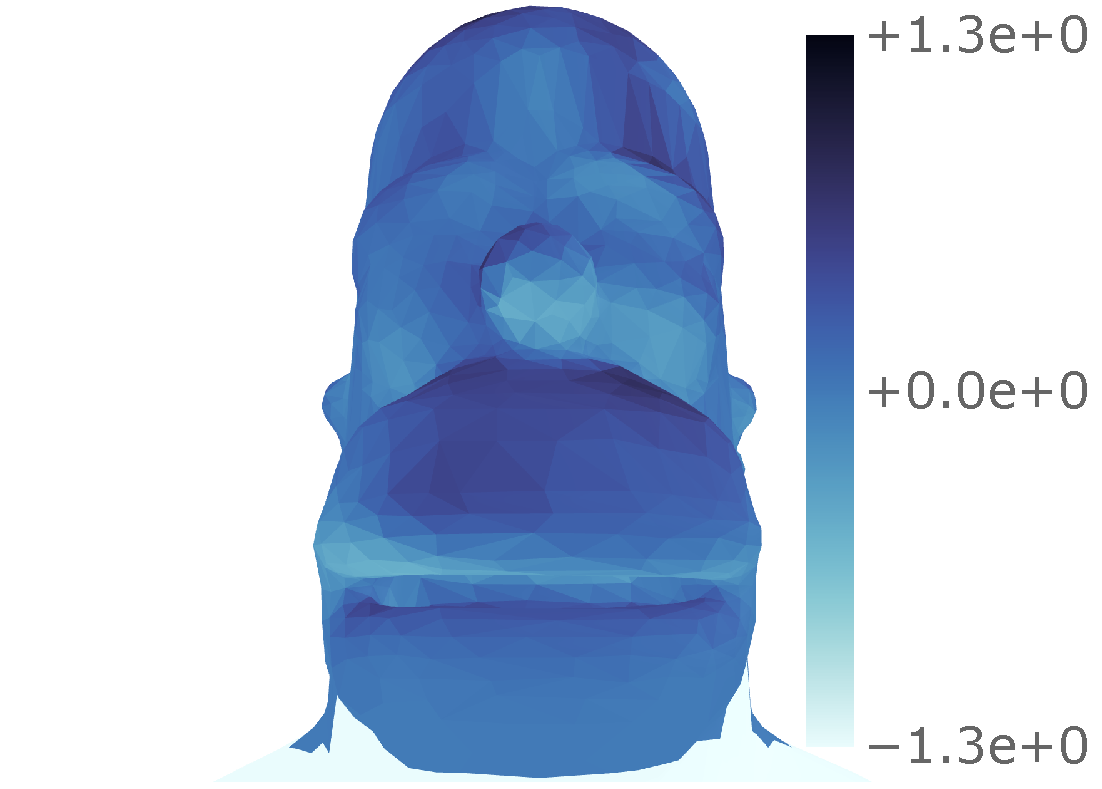
\includegraphics[trim={101 0 3 3},clip,width=.33\textwidth]{slepian_wavelet_coefficients_homer_3B_2jmin_4j_zoom.pdf}}
	\hfill
	\subfloat[\(\mesh{W^{\Psi^{5j}}}\)]
	{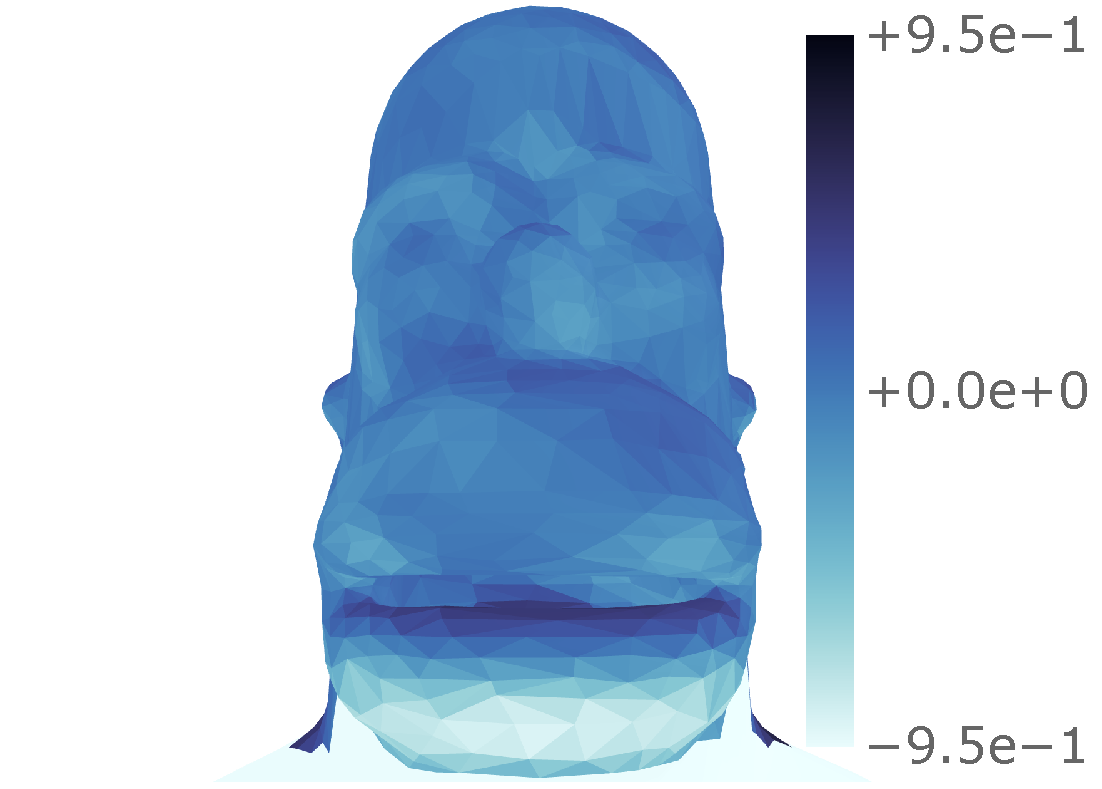
\includegraphics[trim={101 0 3 3},clip,width=.33\textwidth]{slepian_wavelet_coefficients_homer_3B_2jmin_5j_zoom.pdf}}
	\hfill
	\subfloat[\(\mesh{W^{\Psi^{6j}}}\)]
	{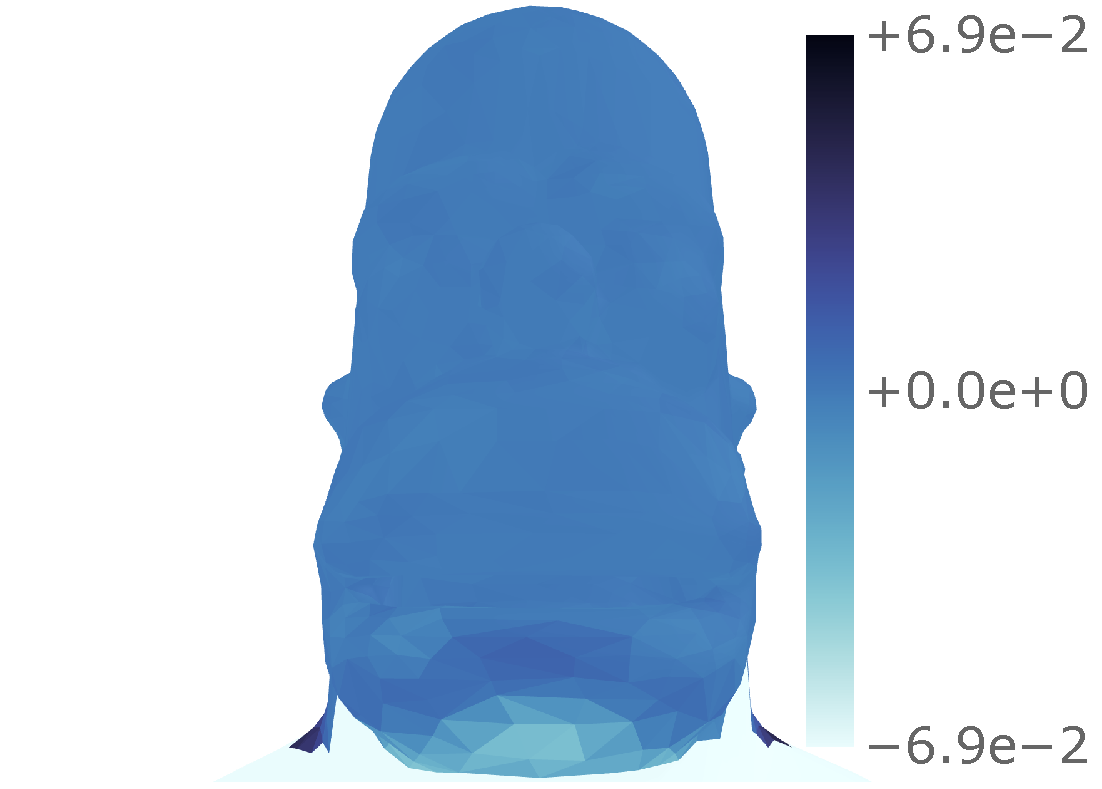
\includegraphics[trim={101 0 3 3},clip,width=.33\textwidth]{slepian_wavelet_coefficients_homer_3B_2jmin_6j_zoom.pdf}}
	\caption{
		The scale-discretised wavelet transform of the per vertex normals of the Homer head region for parameters \(\lambda=3\), \(J_{0}=2\), and \(\num{1275}\) basis functions; \ie{} with the wavelets shown in \cref{fig:chapter4_wavelets}.
		Spatially localised, scale-dependent features of the bandlimited signal may be extracted by the wavelet coefficients given by the wavelet transform.
		The scaling coefficients are given in the top left plot, while the wavelet coefficients at scales \(j \in \set{2, 3, 4, 5, 6}\) are shown left-to-right, top-to-bottom.
	}\label{fig:chapter4_wavelet_coefficients}
\end{figure}
